%===============
%一行目に必ず必要
%文章の形式を定義
%===============
\documentclass{ujarticle}
%===============
%パッケージの定義、必要か不明
%===============
%この下4つを加えることで、mathbbが機能した
\usepackage{amsthm}
\usepackage{amsmath}
\usepackage{amssymb}
\usepackage{amsfonts}
%可換図式用パッケージ
\usepackage{amscd}
\usepackage[all]{xy}
%tilkz用
\usepackage[dvipdfmx]{graphicx}
\usepackage{tikz}
\usepackage{tikz-cd}
\usepackage{my-default}
%リンク用パッケージ
\usepackage[dvipdfmx]{hyperref}
%複数行コメント


\renewenvironment{itemize}%
{%
   \begin{list}{\parbox{1zw}{$\bullet$}}% 見出し記号/直後の空白を調節
   {%
      \setlength{\topsep}{0zh}
      \setlength{\itemindent}{0zw}
      \setlength{\leftmargin}{2zw}%  左のインデント
      \setlength{\rightmargin}{0zw}% 右のインデント
      \setlength{\labelsep}{1zw}%    黒丸と説明文の間
      \setlength{\labelwidth}{3zw}%  ラベルの幅
      \setlength{\itemsep}{0em}%     項目ごとの改行幅
      \setlength{\parsep}{0em}%      段落での改行幅
      \setlength{\listparindent}{0zw}% 段落での一字下り
   }
}{%
   \end{list}%
}





\begin{document}
前半に論文そのものの解説を述べる.

その後,全体に関する考察をする.

\section{Introduction and Crystal Basis Model}
\label{sec:Introduction and Crystal Basis Model}

\section{PART 1: A Minimum Principle in Codon-Anticodon
Interaction}
\label{sec:PART 1: A Minimum Principle in Codon-Anticodon
Interaction}
DNAからタンパク質への翻訳,遷移は複雑なプロセスを経ている.
そのキーとなる箇所がmRNAのヌクレオチドからアミノ酸に変換されるとこである.
\begin{yodan}
 ヌクレオチド同士の物理的な構造はどうなっている?mRNAは完全に(二重らせんの)直線だと思っていいのか?
\end{yodan}
コドンからアンチコドンへ変換され,アンチコドンからアミノ酸に変換される.
コドンは60種類あり,Watoson-Crickの原理を考えると,アンチコドンは60種類あるべきだが,どうやら
60種類より少ないことがわかってきた.
これは1960年台にはわかっており,それを解消する説として,クリックがwobble hypothesisを唱えた.
これは,コドンの3番目の値があまり意味をもたず?一つ目と二つ目だけで対応するアンチコドンが決定されるというものであった.
これは比較的うまくいったが,「何個のアンチドンが必要か」という疑問が生まれた.
これを明らかにするため,以下の仮説が提唱されている.
\begin{enumerate}
  \item The conventional wobble versatility hypothesis assumes that the the first position
  of anticodon should have G (U) to read for codon with Y (respectively R) in third position.
  \item The codon adaptation hypothesis states that the first position of anticodon
  should pair the most abondant codon in the family of synonymous codons
\end{enumerate}
ミトコンドリアで調べてみた結果,正しくタンパク質に変換するためには,最低22個のアンチコドンが必要なことがわかった.
\begin{yodan}
 その後ろ翻訳できねぇ
\end{yodan}

\section{The “minimum” principle}
\label{sec:The “minimum” principle}
Given a codon XYZ (X, Y, Z ∈ \{C, A, G, U\})
we conjecture that an anticodon $X_aY_aZ_a$
, where
$Y_aZ_a = Y_cX_c$, denoting the nucleotide complementary
to the nucleotide N according to the Watson-Crick pairing rule3
, pairs to the codon XYZ, i.e. it is most used to “read” the codon XY Z
if it minimizes the operator T , explicitly written in eq.(2) and computed between the “states”, which
can be read from Table 1, describing the codon and anticodon in the “crystal basis model”. We write
both codons (c) and anticodons (a) in 5” → 3” direction. As an anticodon is antiparallel to codon,
the 1st nucleotide (respectively the 3rd nucleotide) of the anticodon is paired to the 3rd (respectively
the 1st) nucleotide of the codon, see Figure 1


\part{数学についての補足}
\label{pa:数学についての補足}

今回使う数学について説明する.
具体的には以下を説明する.
\begin{itemize}
  \item 有限群とその表現
  \item 表現論から見たフーリエ解析
  \item リー群とその表現
  \item リー環とその表現
  \item 具体的なリー群とリー環の例
  \item Hopf代数
  \item 量子群
  \item crystal basis
\end{itemize}
もう少し具体的には,
- 多様体かつ群ならば局所的にGLしかないこと.
- リー環は一般的に定義できるが,リー群から自然にリー環が定義され,
そのリー環の同型からリー群が決定できること.
- リー環には普遍包絡環が定義できること
- リー群が誘導するリー環は接ベクトル空間とまた,その普遍包絡環はリー群の左不変微分作用素(ベクトル場)と一致すること
それが包絡という意味.
- 量子群の定義
- 量子群の表現
  - 既約表現の決定
  - 完全可約性

今回はリー群,リー環は具体的なものしかみない.

\section{有限群とその表現}
\label{sec:有限群とその表現}

\begin{prop}
 有限群$G$の任意の表現は完全可約である.
\end{prop}

\begin{prop}
 有限アーベル群$G$の任意の既約表現は1次元表現になる.
\end{prop}



\section{リー群とリー環}
\label{sec:リー群とリー環}
リー群とリー環について説明する.リー群とリー環については説明を一番詳しい教科書である
\cite{KO}を参考にしている.そのため,リー群の定義も多様体であって群であるとするのではなく,
局所的に$\mathrm{GL}(n,\mathbb{C})$の部分群になっていることで定義した.(両者は一致する)
\begin{dfn}[線形Lie群]
$\mathrm{GL}(n,\mathbb{C})$の閉部分群を線形Lie群という.
\end{dfn}

\begin{dfn}[局所同型]
位相群$G,H$が局所同型とは,$G,H$の単位元の近傍$V,U$が存在し,
同相写像$\iota:V \to U$であって,$x,y \in V$に対し,
\begin{align*}
  xy \in V  \Leftrightarrow & \iota(x)\iota(y) \in U \\
  xy \in V  \Rightarrow & \iota(x)\iota(y)=\iota(xy)
\end{align*}
\end{dfn}

\begin{dfn}[リー群]
位相群$G$がリー群とは,$e \in G$の近傍$V$で,$V$が$\mathrm{GL}(n,\mathbb{C})$と局所同型なること
\end{dfn}
\begin{rem}
 リー群は$C^{\omega}$級多様体かつ群であり,群演算が$C^{\omega}$級写像となることとも定義できる.
 上の定義と一致することは重要な結果の一つである.
\end{rem}

\begin{dfn}[リー環]
$\mathcal{G}$がリー環とは,ある体$K$上のベクトル空間であって,
任意の$x,y\in \mathcal{G}$に対し,$[x,y] \in G$が定義され,以下を満たすこと.
\begin{align}
  a[x,y]=[ax,y]=[x,ay] \\
  [x,[y,z]]+[y,[z,x]]+[z,[x,y]]=0
\end{align}
\end{dfn}

線形リー群$G$に対し、自然にリー環$\mathcal{G}$が定義される.
\begin{prop}
 線形リー群$G$に対し、$\mathcal{G}:=\{g \in M(n,\mathbb{C})\mid $任意の$t$に対し,
 $\mathrm{exp}(tg) \in G\}$ はリー環になる.
\end{prop}

\begin{epl}
リー群$SL(2,\mathbb{C})$が誘導するリー環$sl(2,\mathbb{C})$は
$\{ g \in M(2,\mathbb{C}) | \mathrm{Tr}g = 0 \}$
と一致する。
\end{epl}
\begin{proof}
 計算すればいい
\end{proof}

\subsection{普遍包絡環}
\label{sub:普遍包絡環}

定義と性質のみ?


リー群の表現はちょっと保留


\section{Hopf代数}
\label{sub:Hopf代数}
ここでは,Hopf代数の定義を記述し,以下2つを示す.
\begin{itemize}
  \item 群$G$から体$K$への写像全体の集合がHopf代数になること
  \item リー環の普遍包絡環がHopf代数になっていること
\end{itemize}

\subsection{Hopf代数の定義}
\label{sub:Hopf代数の定義}
\begin{dfn}
代数$(A,m,\mu)$とは$\mathbb{C}$上のベクトル空間$A$と
\begin{eqnarray*}
m :& A \otimes A \to A  &\mbox{積} \\
\mu :& \mathbb{C} \to A &\mbox{単位射}
\end{eqnarray*}
に対し,以下の図式が可換になること.


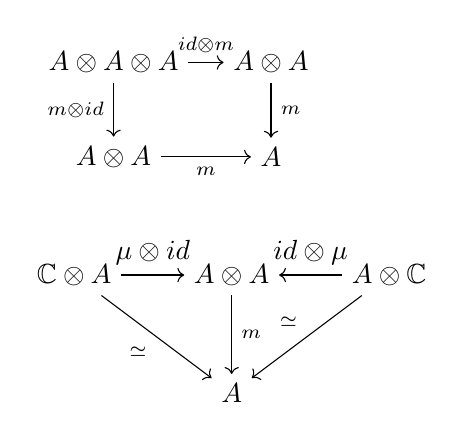
\begin{tikzpicture}[auto]
\node (a) at (2.5, 4.2) {$A \otimes A \otimes A$}; \node (x) at (4.5, 4.2) {$A \otimes A$};
\node (b) at (2.5, 3) {$A \otimes A$};   \node (y) at (4.5, 3) {$A$};
\draw[->] (a) to node {$\scriptstyle id \otimes m$} (x);
\draw[->] (x) to node {$\scriptstyle m$} (y);
\draw[->] (a) to node[swap] {$\scriptstyle m \otimes id $} (b);
\draw[->] (b) to node[swap] {$\scriptstyle m$} (y);

\node (aa) at (2, 1.5) {$\mathbb{C} \otimes A $}; \node (xx) at (4, 1.5) {$A \otimes A$};
\node (zz) at (6,1.5) {$A \otimes \mathbb{C}$};
\node (bb) at (4, 0) {$A$};
\draw[->] (aa) to node {$\mu \otimes id$} (xx);
\draw[->] (zz) to node[swap] {$id \otimes \mu$} (xx);
\draw[->] (xx) to node {$\scriptstyle m$} (bb);
\draw[->] (aa) to node[swap] {$\scriptstyle \simeq$} (bb);
\draw[->] (zz) to node[swap] {$\scriptstyle \simeq$} (bb);
\end{tikzpicture}

\end{dfn}
\begin{rem}
 数式が相変わらず汚い.
\end{rem}
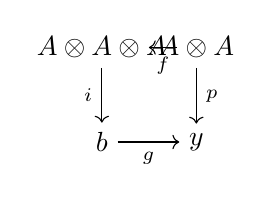
\begin{tikzpicture}[auto]
\node (a) at (0, 1.2) {$A \otimes A \otimes A$}; \node (x) at (1.2, 1.2) {$A \otimes A$};
\node (b) at (0, 0) {$b$};   \node (y) at (1.2, 0) {$y$};
\draw[->] (a) to node {$\scriptstyle f$} (x);
\draw[->] (x) to node {$\scriptstyle p$} (y);
\draw[->] (a) to node[swap] {$\scriptstyle i$} (b);
\draw[->] (b) to node[swap] {$\scriptstyle g$} (y);
\end{tikzpicture}

\begin{prop}
 体$K$と群$G$に対し,$\mathrm{Map}(G,K)$はHopf代数になる.
\end{prop}
\begin{proof}
 はじめに$\mathrm{Map}(G,K) \otimes \mathrm{Map}(G,K) \simeq \mathrm{Map}(G\times G,K)$
 であることを示す.
 $\mathrm{Map}(G,K)$は$K$の直和なので,
\end{proof}

%\section{SLの場合の量子群}
\section{$\mathrm{SL}(2,\mathbb{C})$の場合の量子群}

リー群$\mathrm{SL}(2,\mathbb{C})$に対し,リー環,普遍包絡環を求め,
これを基に量子群を求める.

また,量子群に対する既約表現を決定し,完全可約性を示す.


\begin{thebibliography}{99}
  \bibitem{KO} 小林俊行,大島利雄 リー群と表現 岩波書店(2005/4/6)
  \bibitem{aaa}  ……
\end{thebibliography}

\end{document}
